\documentclass[conference,a4paper]{IEEEtran}
% Built on the IEEE conference template (version 06/27/2024) supplied with this project.
% All numbers are macros from numbers.tex, generated by analysis/06_paper_exps/gen_numbers.py.
\usepackage{cite}
\usepackage{amsmath,amssymb,amsfonts}
\usepackage{graphicx}
\usepackage{textcomp}
\usepackage{xcolor}
\usepackage{booktabs}
\usepackage{tikz}
\usetikzlibrary{positioning,arrows.meta}
\usepackage[hidelinks]{hyperref}
% Auto-generated by analysis/06_paper_exps/gen_numbers.py -- do not edit by hand
\newcommand{\NDpairs}{15{,}101}
\newcommand{\NDshare}{80.3}
\newcommand{\NDgroups}{2{,}782}
\newcommand{\NDmulti}{1{,}004}
\newcommand{\NDcap}{250}
\newcommand{\NDcross}{7}
\newcommand{\NDshareResA}{73.0}
\newcommand{\NDshareResB}{2.9}
\newcommand{\NDshareResC}{90.5}
\newcommand{\NDshareResD}{32.0}
\newcommand{\NDshareResE}{42.1}
\newcommand{\LeakOurs}{0.0}
\newcommand{\LeakMinOurs}{0.0}
\newcommand{\LeakMaxOurs}{0.0}
\newcommand{\PairsOurs}{15{,}101}
\newcommand{\LargestOurs}{204}
\newcommand{\GroupsOurs}{2{,}266}
\newcommand{\LeakPhSix}{69.0}
\newcommand{\LeakMinPhSix}{67.9}
\newcommand{\LeakMaxPhSix}{69.9}
\newcommand{\PairsPhSix}{678}
\newcommand{\LargestPhSix}{55}
\newcommand{\GroupsPhSix}{6{,}682}
\newcommand{\LeakPhEight}{66.8}
\newcommand{\LeakMinPhEight}{65.8}
\newcommand{\LeakMaxPhEight}{68.1}
\newcommand{\PairsPhEight}{2{,}103}
\newcommand{\LargestPhEight}{264}
\newcommand{\GroupsPhEight}{6{,}098}
\newcommand{\LeakPhTen}{66.0}
\newcommand{\LeakMinPhTen}{65.1}
\newcommand{\LeakMaxPhTen}{66.9}
\newcommand{\PairsPhTen}{6{,}251}
\newcommand{\LargestPhTen}{929}
\newcommand{\GroupsPhTen}{5{,}209}
\newcommand{\LeakCosNF}{66.3}
\newcommand{\LeakMinCosNF}{64.7}
\newcommand{\LeakMaxCosNF}{68.3}
\newcommand{\PairsCosNF}{804}
\newcommand{\LargestCosNF}{10}
\newcommand{\GroupsCosNF}{6{,}540}
\newcommand{\LeakCosNinety}{42.4}
\newcommand{\LeakMinCosNinety}{41.6}
\newcommand{\LeakMaxCosNinety}{43.3}
\newcommand{\PairsCosNinety}{11{,}082}
\newcommand{\LargestCosNinety}{626}
\newcommand{\GroupsCosNinety}{3{,}632}
\newcommand{\LeakRand}{69.8}
\newcommand{\LeakMinRand}{67.6}
\newcommand{\LeakMaxRand}{71.8}
\newcommand{\PairsRand}{0}
\newcommand{\LargestRand}{1}
\newcommand{\GroupsRand}{7{,}101}
\newcommand{\RecallPhTen}{7.5}
\newcommand{\RecallPhSix}{2.3}
\newcommand{\RecallCosNinety}{36.1}
\newcommand{\AudOursWeakLo}{11}
\newcommand{\AudOursWeakHi}{12}
\newcommand{\AudOursWeakN}{20}
\newcommand{\AudOursStrongLo}{14}
\newcommand{\AudOursStrongHi}{17}
\newcommand{\AudOursStrongN}{20}
\newcommand{\AudPhOnlyLo}{0}
\newcommand{\AudPhOnlyHi}{9}
\newcommand{\AudPhOnlyN}{20}
\newcommand{\AudCosOnlyLo}{5}
\newcommand{\AudCosOnlyHi}{8}
\newcommand{\AudCosOnlyN}{20}
\newcommand{\AudAccLo}{64}
\newcommand{\AudAccHi}{75}
\newcommand{\LeakValGroupMax}{0.19}
\newcommand{\InjAnchors}{392}
\newcommand{\InjTwins}{395}
\newcommand{\InjA}{197}
\newcommand{\InjB}{195}
\newcommand{\InjBoxesHalf}{581}
\newcommand{\GroupFifty}{0.198}
\newcommand{\GroupFiftySd}{0.015}
\newcommand{\GroupFiftyN}{3}
\newcommand{\GroupFiftyNF}{0.086}
\newcommand{\GroupFiftyNFSd}{0.005}
\newcommand{\GroupFiftyNFN}{3}
\newcommand{\GroupAPLong}{0.282}
\newcommand{\GroupAPLat}{0.220}
\newcommand{\GroupAPAlli}{0.219}
\newcommand{\GroupAPPot}{0.193}
\newcommand{\GroupAPOth}{0.074}
\newcommand{\RandomFifty}{0.219}
\newcommand{\RandomFiftySd}{0.004}
\newcommand{\RandomFiftyN}{3}
\newcommand{\RandomFiftyNF}{0.100}
\newcommand{\RandomFiftyNFSd}{0.003}
\newcommand{\RandomFiftyNFN}{3}
\newcommand{\RandomAPLong}{0.305}
\newcommand{\RandomAPLat}{0.253}
\newcommand{\RandomAPAlli}{0.244}
\newcommand{\RandomAPPot}{0.206}
\newcommand{\RandomAPOth}{0.087}
\newcommand{\InflFifty}{0.021}
\newcommand{\InflFiftyRel}{11}
\newcommand{\InflFiftySd}{0.016}
\newcommand{\InflFiftyMin}{0.007}
\newcommand{\InflFiftyMax}{0.039}
\newcommand{\InflFiftyNF}{0.014}
\newcommand{\InflFiftyNFRel}{16}
\newcommand{\InflFiftyNFSd}{0.008}
\newcommand{\InflFiftyNFMin}{0.006}
\newcommand{\InflFiftyNFMax}{0.022}
\newcommand{\GroupSrcC}{0.198}
\newcommand{\GroupSrcA}{0.107}
\newcommand{\GroupSrcD}{0.225}
\newcommand{\GroupSrcE}{0.187}
\newcommand{\RandomSrcC}{0.216}
\newcommand{\RandomSrcA}{0.150}
\newcommand{\RandomSrcD}{0.199}
\newcommand{\RandomSrcE}{0.155}
\newcommand{\InjLeaked}{0.211}
\newcommand{\InjUnleaked}{0.210}
\newcommand{\InjBase}{0.224}
\newcommand{\InjDiff}{0.001}
\newcommand{\InjDiffLo}{-0.015}
\newcommand{\InjDiffHi}{0.017}
\newcommand{\InjDiffRel}{1}
\newcommand{\InjUB}{-0.014}
\newcommand{\InjUBLo}{-0.028}
\newcommand{\InjUBHi}{0.003}
\newcommand{\PlacDiff}{0.013}
\newcommand{\PlacDiffLo}{0.000}
\newcommand{\PlacDiffHi}{0.026}
\newcommand{\PlacTB}{0.003}
\newcommand{\PlacTBLo}{-0.010}
\newcommand{\PlacTBHi}{0.015}
\newcommand{\NPlacebo}{866}
\newcommand{\NAnchorBoxes}{1162}
\newcommand{\InjClsLong}{0.013}
\newcommand{\InjClsLongLo}{-0.017}
\newcommand{\InjClsLongHi}{0.037}
\newcommand{\InjClsLat}{-0.008}
\newcommand{\InjClsLatLo}{-0.045}
\newcommand{\InjClsLatHi}{0.024}
\newcommand{\InjClsAlli}{0.033}
\newcommand{\InjClsAlliLo}{-0.006}
\newcommand{\InjClsAlliHi}{0.078}
\newcommand{\InjClsPot}{-0.012}
\newcommand{\InjClsPotLo}{-0.033}
\newcommand{\InjClsPotHi}{0.013}
\newcommand{\InjClsOth}{-0.020}
\newcommand{\InjClsOthLo}{-0.063}
\newcommand{\InjClsOthHi}{0.016}
\newcommand{\PrevStrong}{69.3}
\newcommand{\PrevWLo}{71.7}
\newcommand{\PrevWHi}{75.0}
\newcommand{\LeakRandStrong}{56.6}
\newcommand{\LeakRandStrongMin}{56.2}
\newcommand{\LeakRandStrongMax}{57.5}
\newcommand{\LeakRandWLo}{58.7}
\newcommand{\LeakRandWHi}{62.8}
\newcommand{\PlainCCLargest}{808}
\newcommand{\TwinDirectPct}{71}
\newcommand{\TwinMean}{2.0}
\newcommand{\GroupTestSingleton}{41}
\newcommand{\RandTestSingleton}{21}
\newcommand{\RandTestBigGroups}{34}
\newcommand{\GroupTestMaxGroup}{19}
\newcommand{\GroupTrainGroups}{1{,}015}
\newcommand{\RandTrainGroups}{1{,}781}
\newcommand{\LabeledGroups}{2{,}266}
\newcommand{\OverlapGroupLo}{34}
\newcommand{\OverlapGroupHi}{39}
\newcommand{\OverlapRandLo}{14}
\newcommand{\OverlapRandHi}{16}
\newcommand{\GroupCosNinetyShare}{15}
\newcommand{\RandCosNinetyShare}{51}
\newcommand{\ResidLo}{4}
\newcommand{\ResidHi}{6}
\newcommand{\AudFP}{11}
\newcommand{\AudFPNeighbor}{8}
\newcommand{\LeakFullNinety}{39.7}
\newcommand{\LargestFullNinety}{729}
\newcommand{\LeakAvgA}{34.6}
\newcommand{\LargestAvgA}{73}
\newcommand{\LeakAvgB}{29.6}
\newcommand{\LargestAvgB}{190}
\newcommand{\LeakSOurs}{0.0}
\newcommand{\LeakSPhSix}{55.1}
\newcommand{\LeakSPhEight}{53.7}
\newcommand{\LeakSPhTen}{50.3}
\newcommand{\LeakSCosNF}{52.6}
\newcommand{\LeakSCosNinety}{26.1}
\newcommand{\LeakSRand}{56.6}
\newcommand{\LeakSFullNinety}{24.8}
\newcommand{\LeakSAvgA}{20.0}
\newcommand{\LeakSAvgB}{15.8}
\newcommand{\AudOursStrongUnc}{3}
\newcommand{\AudPhOnlyUnc}{9}
\newcommand{\AudCosOnlyUnc}{3}
\newcommand{\HalfA}{-0.013}
\newcommand{\HalfB}{0.015}
\newcommand{\GroupCIWidth}{0.035}
\newcommand{\RandomCIWidth}{0.040}
% Fallback: any macro used in the paper but not defined above renders as red ??


\begin{document}

\title{Quantifying Near-Duplicate Frame Leakage in Crowdsourced Road Damage Detection with Geometry-Verified Splits}

% Review version (double-blind). For camera-ready, replace with the real author block, e.g.
% \author{\IEEEauthorblockN{Given Name Surname}\IEEEauthorblockA{\textit{dept.}\\\textit{organization}\\City, Indonesia\\e-mail or ORCID}}
\author{\IEEEauthorblockN{Anonymous Authors}
\IEEEauthorblockA{Paper under double-blind review}}

\maketitle

\begin{abstract}
Road damage datasets are often built from video frames recorded on moving vehicles, producing many near-duplicate images. A random split then places the same road spot in training and test sets, so the test score no longer measures generalization to unseen roads. We audit this leakage in RDDC2024-ID, a crowdsourced Indonesian dataset of 9,048 frames, captured mostly from motorcycles, with five damage classes. We propose a near-duplicate grouping protocol for two confounders of road video, the visible ego vehicle and repetitive pavement texture: self-supervised embeddings retrieve candidate pairs, local-feature matching on the upper part of the frame verifies them after discarding static matches, and a chaining-resistant rule forms groups for a stratified split. Between \PrevStrong{} and \NDshare{} percent of the images have a near-duplicate, and a random split leaks one for \LeakRand{} percent of test images, while grouping by perceptual hashing still leaves \LeakPhTen{} to \LeakPhSix{} percent leaked. Across three split draws, a YOLO11n detector scores \InflFifty{} mAP50 (\InflFiftyRel{} percent) higher on random than on group-aware splits, with the gap varying between draws. A crossover experiment that moves near-duplicates of fixed held-out images into training, without changing the amount of training data, changes their mAP50 by only \InjDiff{}, with a confidence interval that includes zero. Leakage thus invalidates random splits, but its effect on the score of a lightweight detector is modest and comparable to the variation between draws. We release the split lists and code.
\end{abstract}

\begin{IEEEkeywords}
road damage detection, data leakage, near-duplicate detection, dataset splitting, object detection, Indonesia
\end{IEEEkeywords}

\section{Introduction}
Automatic road damage detection from low-cost cameras is a practical way for road agencies to survey large networks. Public benchmarks such as RDD2020, which covers three countries \cite{arya2021rdd2020}, its six-country extension RDD2022 \cite{arya2024rdd2022}, and the CRDDC'2022 challenge built on the latter \cite{arya2022crddc}, collect images mostly with vehicle-mounted smartphones; its successor ORDDC'2024 added inference speed to the ranking \cite{arya2024orddc}, and recent detectors are trained and compared on such data \cite{lin2025striprfnet}. A cheap way to grow a dataset is to record video and extract frames. Consecutive frames, however, show the same road spot from almost the same viewpoint. When frames are split into training and test sets at random, near-duplicates end up on both sides and the test score partly measures recognition of seen locations.

\begin{figure*}[t]
\centering
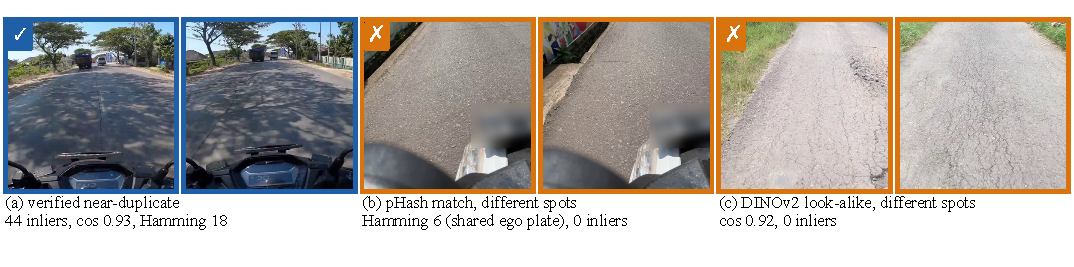
\includegraphics[width=\textwidth]{figs/fig_pairs.pdf}
\caption{Candidate pairs in RDDC2024-ID. Labels give moving SIFT inliers, DINOv2 cosine similarity (cos) and pHash Hamming distance. (a) A geometrically verified near-duplicate from the same ride that perceptual hashing misses (Hamming distance 18). (b) A pair from the down-looking 1080-pixel source that perceptual hashing matches (Hamming distance 6) only because the ego vehicle and its license plate (blurred) occupy the same pixels; the road spots differ. (c) Two different spots with look-alike pavement above a DINOv2 cosine threshold of 0.90.}
\label{fig:pairs}
\end{figure*}

This form of leakage is documented outside road damage. Near-duplicates inflated license plate recognition results and changed model rankings \cite{laroca2023duplicates}; revisited locations inflated online-mapping scores, for some methods by more than 45 mAP \cite{lilja2024localization}; correlated video frames leaked across splits of object detection datasets \cite{figueiredo2024leakage}, which cluster-based splitting was later designed to prevent \cite{glazner2026findleak}; and leakage in general is a recognized cause of irreproducible machine-learning results \cite{kapoor2023leakage}. In automotive perception, leaking test images into training raised detector mAP steeply, and similar images were found with perceptual hashing \cite{babu2024leakage}. For road damage, a recent Indonesian pothole video dataset is split by video \cite{ihsan2024pothole}, but, to our knowledge, no study has measured how much near-duplicate leakage affects road damage detection results.

Road video has two properties that make generic de-duplication fail. First, the camera is fixed to the vehicle, so the fairing, headlight, dashboard or license plate occupies the same pixels in every frame and makes unrelated frames look alike. Second, asphalt and concrete are repetitive textures, so appearance embeddings match different spots that merely look similar (Fig.~\ref{fig:pairs}).

We study this problem on RDDC2024-ID, a crowdsourced Indonesian dataset whose 44 contributors extracted frames from road videos, labeled them and cross-validated the annotations; it has five classes and several capture setups but is released without an official split \cite{rddc2024id}, so every study that uses it has to define its own. Road damage research has so far treated shifts between countries and devices, through domain adaptation \cite{lin2023dardd} and self-supervised visual prompting for cross-domain detection \cite{xiao2026probe}, rather than leakage inside one dataset. Among leakage studies, the cluster-based splits of Glazner et~al.\ compare embedding families by clustering quality without training detectors \cite{glazner2026findleak}, and the automotive injection study adds exact test copies without controlling for the amount of added data \cite{babu2024leakage}. We find hashing confounded by the ego vehicle and global embeddings by pavement texture, so we adapt the spatial verification long used for near-duplicate retrieval \cite{philbin2007spatial} to a camera fixed to the vehicle, measure the residual leakage of each grouping rule, and control the injection experiment with a crossover design. Our contributions are:
\begin{itemize}
\item a leakage audit of a video-derived road damage dataset: \NDshare\% of its images have an accepted near-duplicate (\PrevStrong\% with high-confidence pairs only), and in a random split \LeakRand\% of test images have one in training (\LeakRandStrong\% with high-confidence pairs);
\item a near-duplicate grouping protocol designed for ego-vehicle occlusion and pavement texture, compared with perceptual-hash, embedding-threshold and embedding-clustering grouping by residual leakage and by a stratum-blinded visual audit;
\item a measurement of the effect on detector evaluation over three split draws (random splits score \InflFifty{} mAP50 higher), and a crossover twin-injection experiment that separates the effect of having an image's own near-duplicate group in training from the effect of adding the same amount of data, which finds no detectable anchor-specific gain for a lightweight detector;
\item split lists, grouping code and per-source baselines, to be released with the paper.
\end{itemize}

\section{Methods}
\subsection{Dataset}
RDDC2024-ID contains 9,048 square images, of which 7,101 carry YOLO-format labels with 20,211 boxes in five classes: longitudinal crack (5,127), lateral crack (3,432), alligator crack (3,675), pothole (6,249) and others (1,728). The remaining 1,947 images have no label file; a visual check of 40 of them suggests that most (about 88\%) show no damage, so we exclude them from training and evaluation but keep them in the near-duplicate grouping. The capture devices are not documented, but by visual inspection most frames were recorded from motorcycles. The five image resolutions broadly correspond to capture setups, and we call each resolution a \textit{source} (Table~\ref{tab:sources}): mostly forward-looking cameras on sport and adventure motorcycles (960 and 640 pixels; the 960-pixel source also contains tilted-down and close-up frames, and 256 of the 640-pixel frames come from a down-looking rig), down-looking rigs that see the headlight and, at 1080 pixels, the license plate (1080 and 720 pixels), and a top-down city rig (1600 pixels). A linear probe on DINOv2 features of images resized to 224 pixels identifies the source with 0.985 balanced accuracy under five-fold cross-validation with near-duplicate groups kept within folds, and with 0.981 when only the upper 60\% of the frame is used, so the sources differ strongly in appearance and not only in pixel count.

\begin{table}[t]
\caption{Sources in RDDC2024-ID (fwd.: forward-looking; down: down-looking). ND: share of images with at least one accepted near-duplicate. Ego: share of frames showing the ego vehicle (visual check of a stratified sample).}
\label{tab:sources}
\centering
\setlength{\tabcolsep}{3.3pt}
\begin{tabular}{@{}lrrrrrr@{}}
\toprule
Source (px) & Images & Labeled & Boxes & Box/img & ND\% & Ego\%\\
\midrule
960, mostly fwd. & 6,047 & 5,025 & 15,515 & 3.09 & \NDshareResC & 29\\
640, mostly fwd. & 2,032 & 1,268 & 2,812 & 2.22 & \NDshareResA & 25\\
1080, down & 525 & 428 & 1,031 & 2.41 & \NDshareResD & 100\\
1600, top-down & 340 & 302 & 688 & 2.28 & \NDshareResE & 12\\
720, down & 104 & 78 & 165 & 2.12 & \NDshareResB & 100\\
\midrule
Total & 9,048 & 7,101 & 20,211 & 2.85 & \NDshare & 32\\
\bottomrule
\end{tabular}
\end{table}

\subsection{Geometry-Verified Grouping}
Our protocol has three stages followed by a stratified split (Fig.~\ref{fig:pipeline}).

\textit{Candidate retrieval.} Each image is embedded with DINOv2 ViT-S/14 \cite{oquab2024dinov2} computed on its upper 60\%, which removes most of the ego vehicle. For every image we keep its 15 nearest neighbors with cosine similarity of at least 0.75, which yields 88,619 candidate pairs. Pairs outside this set are never verified, so our counts are lower bounds.

\textit{Geometric verification.} We resize each image to a width of 480 pixels, crop its upper 60\%, and extract up to 1,000 SIFT features \cite{lowe2004sift} with RootSIFT normalization. Only keypoints in the upper half of the full frame are kept, which excludes the license plates and headlights of the down-looking sources. Descriptors are matched with Lowe's ratio test (0.8). Matches that move less than 4 pixels at this working width are discarded, because static matches come from the ego vehicle or from video overlays, not from the scene. A fundamental matrix is fitted to the remaining matches with MAGSAC++ \cite{barath2020magsac} at a 1.5-pixel threshold. A pair is accepted if it has at least 15 moving inliers, or if its embedding similarity is at least 0.96 (26 pairs are accepted by similarity alone). The inlier threshold was calibrated by inspecting pairs from successive inlier bands and deliberately set permissive: a false merge only makes a split stricter, whereas a missed pair leaks.

\textit{Chaining-resistant grouping.} Plain connected components of all accepted pairs would form a group of \PlainCCLargest{} images. Strong edges (at least 30 inliers, or similarity of at least 0.96) are always used; weaker edges are used only if the two images share a verified neighbor (triangle support) or if one of them has no other edge (leaf rule). The held-back weak edges are then merged, strongest first, as long as the merged group does not exceed \NDcap{} images; 38 merges are refused.

\textit{Stratified group-aware split.} Whole groups are assigned to training, validation and test (70/15/15\%) by a greedy procedure that minimizes the deviation from the target shares of images, of each source and of the box count of each class, followed by local moves. We repeat it with three seeds to obtain three split draws; the random splits use the same ratios without stratification. Because the largest groups always go to training, the group-aware test sets share \OverlapGroupLo--\OverlapGroupHi\% of their images across draws, against \OverlapRandLo--\OverlapRandHi\% for random draws.

\begin{figure}[t]
\centering
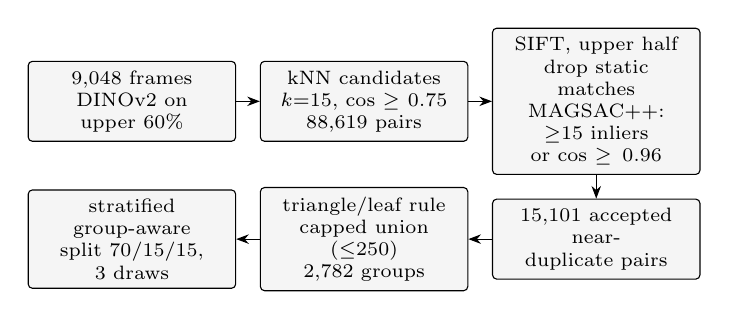
\begin{tikzpicture}[node distance=3mm and 3mm, every node/.style={font=\scriptsize, align=center},
  box/.style={draw, rounded corners=1.5pt, fill=gray!8, minimum height=9mm, text width=24mm}, >={Stealth[length=1.6mm]}]
\node[box] (a) {9,048 frames\\DINOv2 on upper 60\%};
\node[box, right=of a] (b) {kNN candidates\\$k{=}15$, cos $\geq 0.75$\\88,619 pairs};
\node[box, right=of b] (c) {SIFT, upper half\\drop static matches\\MAGSAC++: $\geq$15 inliers\\or cos $\geq 0.96$};
\node[box, below=of c] (d) {\NDpairs{} accepted\\near-duplicate pairs};
\node[box, left=of d] (e) {triangle/leaf rule\\capped union ($\leq$\NDcap)\\\NDgroups{} groups};
\node[box, left=of e] (f) {stratified group-aware\\split 70/15/15, 3 draws};
\draw[->] (a) -- (b); \draw[->] (b) -- (c); \draw[->] (c) -- (d); \draw[->] (d) -- (e); \draw[->] (e) -- (f);
\end{tikzpicture}
\caption{Near-duplicate grouping and group-aware splitting.}
\label{fig:pipeline}
\end{figure}

\subsection{Baseline Grouping Rules and Visual Audit}
\label{sec:baselines}
We apply the same greedy stratified split (60 restarts, three seeds) to groups formed by perceptual hashing of the full frame (pHash; 64-bit DCT hash, Hamming thresholds of 6, 8 and 10, as in \cite{babu2024leakage}), by connected components of DINOv2 similarity thresholds, and by average-linkage clustering of the same embedding cut at a cosine distance of 0.15 or 0.18, in the spirit of the CLIP-based clustering of Figueiredo and Mendes \cite{figueiredo2024leakage}; Glazner et~al.\ compared such embedding families in more detail \cite{glazner2026findleak}. The DINOv2 rules use the upper-60\% embedding of our retrieval stage, so they already benefit from removing the ego vehicle; a full-frame embedding is also tested. We report residual leakage, the share of test images that still have an accepted near-duplicate in training, both against all accepted pairs and against strong pairs only, and the largest group, since a single huge group cannot be stratified. Because residual leakage is measured against our own accepted pairs, it is nearly tautological for our rule; we therefore also checked decisions visually on 80 pairs sampled from four strata (strong and weak accepted pairs, pairs matched only by hashing, and pairs above a 0.90 embedding threshold but rejected by us) and shown in random order without their stratum, by one rater on 300-pixel thumbnails with an ``uncertain'' option; a pair counted as positive only if both frames showed the same road spot.

\subsection{Detector Training and Evaluation}
We train YOLO11n \cite{jocher2024yolo11} (Ultralytics 8.4.75, COCO-pretrained) at 640 pixels for 40 epochs with batch size 16, the default augmentation and optimizer, and training seed 0 for every run, on an RTX 3070 Ti Laptop GPU (8 GB); one run takes about 35 minutes. We did not repeat training with other seeds, so the reported intervals cover test-set sampling but not training variance. For the comparison of three random and three group-aware split draws, the checkpoint is selected on each split's own validation set, and we report the mean average precision at an intersection-over-union (IoU) threshold of 0.5 (mAP50) and averaged over IoU thresholds from 0.5 to 0.95 (mAP50-95), computed by Ultralytics (confidence threshold 0.001, non-maximum suppression IoU 0.7).

\subsection{Crossover Twin Injection}
We fix a population of anchors: one randomly chosen image from each of the \InjAnchors{} multi-image groups in the validation and test sets of the first group-aware split. The anchors are divided into halves A and B (\InjA{} and \InjB{} images, balanced by source and box count, \InjBoxesHalf{} boxes each). Model A is trained on the group-aware training set in which the same \InjTwins{} randomly chosen training images are replaced by \InjTwins{} twins of the A anchors, i.e., other members of their groups (one to five per anchor, \TwinMean{} on average; \TwinDirectPct\% are direct verified near-duplicates of their anchor); model B receives the same number of twins of the B anchors instead. Both models thus see the same amount of extra data with matched source composition, and every anchor is evaluated once by the model that saw its twins (leaked) and once by the model that did not (unleaked). A third model trained on the unmodified training set serves as reference. Held-out labeled images without a labeled near-duplicate (\NPlacebo{} singletons), weighted to the anchors' source mix, serve as a placebo that neither model has leaked. Because the anchors come from the validation and test sets, we use the final checkpoint without validation-based selection, and compute AP50 with our own implementation (101-point interpolation, greedy matching at IoU 0.5), which gives values about 6--7\% below Ultralytics on the same predictions but allows paired bootstrap intervals over images (2,000 resamples); we therefore compare only differences. Because each anchor comes from a different group, the bootstrap over anchors is also a group-level bootstrap.

\section{Results}
\subsection{Near-Duplicate Prevalence and Split Leakage}
The protocol accepts \NDpairs{} near-duplicate pairs and forms \NDgroups{} groups, \NDmulti{} of which contain more than one image; \NDshare\% of all images belong to a multi-image group. Prevalence depends on the source (Table~\ref{tab:sources}): it is highest for the 960-pixel source, whose groups are long continuous rides (the largest labeled group has \LargestOurs{} images), and lowest for the 720-pixel source. Only \NDcross{} accepted pairs link different sources, and all of them were false matches on inspection, which indicates that true near-duplicates stay within a source; six of them merged 640- and 960-pixel groups through the capped union, which makes the split stricter, not leakier.

With a random 70/15/15 split, \LeakRand\% of the test images (\LeakMinRand--\LeakMaxRand\% over three draws) have an accepted near-duplicate in the training set. Because accepted pairs are not all true near-duplicates (Section~\ref{sec:audit}), we also count only strong pairs, which gives \LeakRandStrong\% (\LeakRandStrongMin--\LeakRandStrongMax\%), and weighting each pair by its audited precision gives \LeakRandWLo--\LeakRandWHi\%. The group-aware splits have no test image with an accepted near-duplicate in training, and at most \LeakValGroupMax\% of validation images are affected, through the 38 edges refused by the group cap.

\subsection{Comparison With Other Grouping Rules}
\label{sec:audit}
Perceptual hashing hardly helps (Table~\ref{tab:rules}): it leaves \LeakPhTen--\LeakPhSix\% of test images leaked, close to the random split, because it finds only \RecallPhSix--\RecallPhTen\% of the accepted pairs, and loosening the threshold mainly merges frames of the down-looking sources that share the ego vehicle (Fig.~\ref{fig:pairs}(b)). A DINOv2 threshold of 0.90 recovers more pairs (\RecallCosNinety\%) but chains \LargestCosNinety{} labeled images into one group and still leaves \LeakCosNinety\% leakage. Average-linkage clustering avoids chaining (largest group \LargestAvgB) but still leaves \LeakAvgB\%. The ranking is the same against strong pairs only.

In the visual audit, counting uncertain pairs first as negative and then as positive, accepted pairs were positive in \AudOursStrongLo--\AudOursStrongHi{} of 20 strong and \AudOursWeakLo--\AudOursWeakHi{} of 20 weak pairs, an estimated precision of \AudAccLo--\AudAccHi\% over all accepted pairs; \AudFPNeighbor{} of the \AudFP{} false positives connect frames that are also linked through a common verified neighbor, i.e., nearby frames of the same ride. None of the 20 pairs matched by hashing but rejected by us was judged the same spot (\AudPhOnlyUnc{} were uncertain), whereas \AudCosOnlyLo--\AudCosOnlyHi{} of 20 pairs above the 0.90 embedding threshold but rejected by us were positive; two of the clear positives fall just below the inlier threshold and three yield no moving matches. Since \GroupCosNinetyShare\% of our test images have a training neighbor above that threshold (random splits: \RandCosNinetyShare\%), we estimate that \ResidLo--\ResidHi\% of them keep an undetected near-duplicate in training.

\begin{table}[t]
\caption{Grouping rules applied before the same greedy stratified split. Largest group counts labeled images. Leakage: share of labeled test images with an accepted near-duplicate in training, mean over three split draws, against all accepted pairs and against strong pairs only (nearly tautological for our rule; see the audit-based estimate in the text).}
\label{tab:rules}
\centering
\setlength{\tabcolsep}{3.5pt}
\begin{tabular}{@{}lrrr@{}}
\toprule
Grouping rule & Largest & \multicolumn{2}{c}{Leakage (\%)}\\
 & group & all & strong\\
\midrule
None (random split) & 1 & \LeakRand & \LeakSRand\\
pHash, Hamming $\leq 6$ & \LargestPhSix & \LeakPhSix & \LeakSPhSix\\
pHash, Hamming $\leq 8$ & \LargestPhEight & \LeakPhEight & \LeakSPhEight\\
pHash, Hamming $\leq 10$ & \LargestPhTen & \LeakPhTen & \LeakSPhTen\\
DINOv2, cosine $\geq 0.95$ & \LargestCosNF & \LeakCosNF & \LeakSCosNF\\
DINOv2, cosine $\geq 0.90$ & \LargestCosNinety & \LeakCosNinety & \LeakSCosNinety\\
DINOv2 full frame, cosine $\geq 0.90$ & \LargestFullNinety & \LeakFullNinety & \LeakSFullNinety\\
DINOv2 average linkage, cut 0.15 & \LargestAvgA & \LeakAvgA & \LeakSAvgA\\
DINOv2 average linkage, cut 0.18 & \LargestAvgB & \LeakAvgB & \LeakSAvgB\\
Geometry-verified (ours) & \LargestOurs & \LeakOurs & \LeakSOurs\\
\bottomrule
\end{tabular}
\end{table}

\subsection{Random Versus Group-Aware Splits}
\label{sec:e1}
Random splits score \RandomFifty{} $\pm$ \RandomFiftySd{} mAP50 and group-aware splits \GroupFifty{} $\pm$ \GroupFiftySd{} (Table~\ref{tab:results}), a difference (random minus group-aware) of \InflFifty{} (\InflFiftyRel\% relative; \InflFiftyMin{} to \InflFiftyMax{} across draws with the same seed index, which are not paired); for mAP50-95 the difference is \InflFiftyNF{} (\InflFiftyNFRel\%). With three correlated draws per split type we report these differences descriptively. The mAP50 difference has the same sign in every draw, and the mean AP50 is higher on random splits for every class, but individual classes change sign between draws and the overall difference varies by a factor of about five, and the spread among the group-aware draws alone (\GroupFiftySd{} standard deviation) is comparable to the mean difference (Fig.~\ref{fig:results}(a)). The two kinds of split have the same size and similar source mix and class shares, but they differ in more than leakage: group-aware test sets contain no group larger than \GroupTestMaxGroup{} images and \GroupTestSingleton\% singletons (random: \RandTestSingleton\% singletons and \RandTestBigGroups\% of images from groups of 20 or more), and group-aware training sets cover about \GroupTrainGroups{} of the \LabeledGroups{} labeled groups against about \RandTrainGroups{} for random splits. This comparison therefore shows how much a reported number depends on the splitting practice rather than isolating the effect of near-duplicates, which the crossover experiment addresses.

\subsection{Crossover Twin Injection}
On the anchors, mAP50 is \InjLeaked{} when leaked and \InjUnleaked{} when unleaked, a difference of \InjDiff{} (95\% confidence interval, CI, \InjDiffLo{} to \InjDiffHi{}; \InjDiffRel\% relative), and the reference model reaches \InjBase{}. Each half gives its own estimate (A anchors, model A minus model B: \HalfA; B anchors, model B minus model A: \HalfB). On the placebo, models A and B differ by \PlacDiff{} (CI \PlacDiffLo{} to \PlacDiffHi{}), which shows that two models trained on equally sized sets already differ by about 0.01 (Fig.~\ref{fig:results}(b)). The anchor difference is therefore indistinguishable from zero: the two halves disagree in sign and are no larger than the difference between models on the placebo. Replacing \InjTwins{} diverse training images by near-duplicates also did not help the anchors relative to the reference model (unleaked minus reference \InjUB{}, CI \InjUBLo{} to \InjUBHi{}). At a dose of about two twins per anchor, YOLO11n trained for 40 epochs thus shows no detectable memorization of individual road spots.

\begin{figure}[t]
\centering
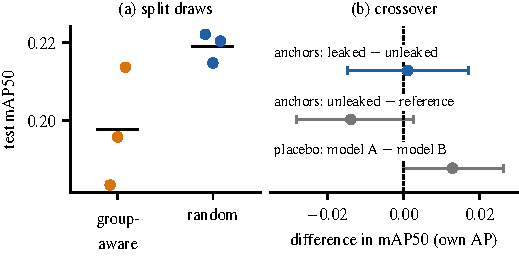
\includegraphics[width=\columnwidth]{figs/fig_results.pdf}
\caption{(a) Test mAP50 of the three group-aware and three random split draws (bars: means; draws are not paired). (b) Crossover twin injection: differences in anchor mAP50 (own implementation) with 95\% bootstrap intervals, and the difference between the two injected models on the placebo images.}
\label{fig:results}
\end{figure}

\begin{table}[t]
\caption{YOLO11n test results. Top: mean $\pm$ standard deviation over three split draws of Ultralytics mAP50, mAP50-95 and per-class AP50 (Long., Lat., Alli.: longitudinal, lateral and alligator crack; Pot.: pothole; Oth.: others). Bottom: crossover twin injection on the anchors, mAP50 from our own implementation (not comparable in absolute terms with the top rows), with the 95\% paired bootstrap interval of the difference; each model was trained once.}
\label{tab:results}
\centering
\setlength{\tabcolsep}{2.4pt}
\begin{tabular}{@{}lccccccc@{}}
\toprule
Split & mAP50 & mAP50-95 & Long. & Lat. & Alli. & Pot. & Oth.\\
\midrule
Random & \RandomFifty{}\scriptsize{$\pm$\RandomFiftySd} & \RandomFiftyNF{}\scriptsize{$\pm$\RandomFiftyNFSd} & \RandomAPLong & \RandomAPLat & \RandomAPAlli & \RandomAPPot & \RandomAPOth\\
Group-aware & \GroupFifty{}\scriptsize{$\pm$\GroupFiftySd} & \GroupFiftyNF{}\scriptsize{$\pm$\GroupFiftyNFSd} & \GroupAPLong & \GroupAPLat & \GroupAPAlli & \GroupAPPot & \GroupAPOth\\
\midrule
\multicolumn{8}{@{}l}{Crossover on \InjAnchors{} anchors (\NAnchorBoxes{} boxes)}\\
\multicolumn{3}{@{}l}{Reference / unleaked / leaked} & \multicolumn{5}{l}{\InjBase{} / \InjUnleaked{} / \InjLeaked{}}\\
\multicolumn{3}{@{}l}{Leaked minus unleaked} & \multicolumn{5}{l}{\InjDiff{} [\InjDiffLo, \InjDiffHi]}\\
\multicolumn{3}{@{}l}{Placebo, model A minus model B} & \multicolumn{5}{l}{\PlacDiff{} [\PlacDiffLo, \PlacDiffHi]}\\
\bottomrule
\end{tabular}
\end{table}

\subsection{Per-Source and Per-Class Behavior}
On group-aware test sets, mAP50 (own implementation, mean over draws) is \GroupSrcC{} for the 960-pixel source, \GroupSrcA{} for 640, \GroupSrcD{} for 1080 and \GroupSrcE{} for 1600; the 1080- and 1600-pixel test sets have only about 64 and 45 images, and the 720-pixel source has too few test images to report. The 640-pixel source, mostly hilly rural roads with soft, possibly upscaled frames, is the hardest in all three draws, and it also gains the most on random splits (\RandomSrcA{} against \GroupSrcA{}). Across classes, others scores lowest in every setting (Table~\ref{tab:results}). An inspection of 120 boxes of the others class found edge breaks, raveling and patching in about one fifth each, and 16\% with unclear or no damage visible at thumbnail resolution. Most errors of the seed-0 group-aware model are missed objects rather than confusions between classes, and small objects (mostly potholes) are rarely detected at 640 pixels.

\section{Discussion and Conclusion}
\label{sec:discussion}
\subsection{Interpretation and Recommendations}
Near-duplicates are the rule rather than the exception in frames extracted from road videos: in RDDC2024-ID, \PrevStrong--\NDshare\% of the images have one, and a random split leaks a near-duplicate of most test images into training. For a lightweight detector, however, the measured effect on the score is modest, and the crossover experiment finds no anchor-specific gain; all runs were still underfitting (training loss decreasing at the last epoch), so larger models or longer schedules may behave differently. The difference between random and group-aware splits therefore appears to reflect the different composition of their test sets more than memorization, and random splits are invalid mainly because they do not measure generalization to unseen roads. For video-derived road damage data, random frame-level splits should not be used for reporting, and perceptual-hash de-duplication should not be assumed to fix them. The ego vehicle should be cropped or masked before similarity is computed (in the down-looking sources, hash matches are dominated by it), local geometric verification reduces confusion between true revisits and look-alike pavement, and groups should be formed with a rule that resists chaining. Results should be reported per source, because an aggregate score can hide large differences between sources, and over several group-aware split draws, because a single draw can move mAP50 by as much as the leakage effect itself.

\subsection{Residual Leakage and Limitations}
Our grouping misses some true near-duplicates, and group-aware test images can still come from the same ride as training images at a different spot. We estimate that \ResidLo--\ResidHi\% of our test images keep an undetected near-duplicate in training, against \LeakRandStrong--\LeakRand\% under a random split. Adding the missed embedding edges would merge groups far beyond our cap (the 0.90 threshold alone chains \LargestCosNinety{} labeled images), so we report them as a limitation instead. Leave-one-source-out evaluation, which is possible because no true near-duplicate pair crosses sources, is a stricter complement. The visual audit used one rater and thumbnails. In forward-looking frames the upper half, where keypoints are kept, shows mostly the far road and roadside, so the verifier detects a shared viewpoint more than a shared road spot, which is consistent with its false positives being nearby frames of the same ride. We used a single lightweight detector with a short schedule and one training seed per configuration; larger models have more capacity to memorize and may be affected more strongly, and with one detector we cannot test whether leakage changes model rankings, as it does for license plate recognition \cite{laroca2023duplicates}. The crossover experiment does not separate memorization of a road spot from adaptation to the same ride, camera and annotator. Labels were produced by many contributors and contain loose boxes and inconsistent use of the others class, which caps absolute accuracy. Some frames show faces and license plates, and a few carry video overlays; we release only split lists and code, not images, and blur plates in figures. For the first split, the release also marks the 1,582 unlabeled images that can be added to training without leakage. The dataset is distributed under the MIT license \cite{rddc2024id}.

\subsection{Conclusion}
Perceptual hashing finds fewer than 8\% of the accepted pairs, and the pairs it adds at looser thresholds mostly share only the ego vehicle. Embedding retrieval with geometric verification on the upper part of the frame and a chaining-resistant grouping rule yields a split without accepted-pair leakage and an estimated residual leakage of \ResidLo--\ResidHi\%. For a lightweight YOLO11n detector, random splits scored \InflFifty{} mAP50 higher than group-aware splits across three draws, while a crossover experiment found no detectable gain from having an image's own near-duplicates in training; the leakage mainly invalidates what a random split measures, and its effect on the score should be judged over several draws. Higher input resolution and small-object heads for potholes are natural next steps on the released group-aware benchmark for Indonesian road damage detection.

\section*{Acknowledgment}
We thank the 44 contributors of RDDC2024-ID for sourcing, labeling and cross-validating the data. % TODO(author): add funding for the camera-ready version

\IEEEtriggeratref{10}  % balance the columns of the last page
\begin{thebibliography}{00}
\bibitem{arya2021rdd2020} D. Arya, H. Maeda, S. K. Ghosh, D. Toshniwal, and Y. Sekimoto, ``RDD2020: An annotated image dataset for automatic road damage detection using deep learning,'' \textit{Data Brief}, vol. 36, Art. no. 107133, 2021, doi: 10.1016/j.dib.2021.107133.
\bibitem{arya2024rdd2022} D. Arya, H. Maeda, S. K. Ghosh, D. Toshniwal, and Y. Sekimoto, ``RDD2022: A multi-national image dataset for automatic road damage detection,'' \textit{Geosci. Data J.}, vol. 11, no. 4, pp. 846--862, 2024, doi: 10.1002/gdj3.260.
\bibitem{arya2022crddc} D. Arya \textit{et al.}, ``Crowdsensing-based road damage detection challenge (CRDDC'2022),'' in \textit{Proc. IEEE Int. Conf. Big Data}, 2022, pp. 6378--6386, doi: 10.1109/BigData55660.2022.10021040.
\bibitem{arya2024orddc} D. Arya, H. Omata, H. Maeda, and Y. Sekimoto, ``ORDDC'2024: State of the art solutions for optimized road damage detection,'' in \textit{Proc. IEEE Int. Conf. Big Data}, 2024, pp. 8430--8438, doi: 10.1109/BigData62323.2024.10825254.
\bibitem{lin2025striprfnet} J. Lin, Y. Qin, S. Gao, Y. Rui, J. Liu, and Y. Lv, ``StripRFNet: A strip receptive field and shape-aware network for road damage detection,'' 2025, arXiv:2510.16115. [Online]. Available: https://arxiv.org/abs/2510.16115
\bibitem{laroca2023duplicates} R. Laroca, V. Estevam, A. S. Britto Jr., R. Minetto, and D. Menotti, ``Do we train on test data? The impact of near-duplicates on license plate recognition,'' in \textit{Proc. Int. Joint Conf. Neural Netw. (IJCNN)}, 2023, pp. 1--8, doi: 10.1109/IJCNN54540.2023.10191584.
\bibitem{lilja2024localization} A. Lilja, J. Fu, E. Stenborg, and L. Hammarstrand, ``Localization is all you evaluate: Data leakage in online mapping datasets and how to fix it,'' in \textit{Proc. IEEE/CVF Conf. Comput. Vis. Pattern Recognit. (CVPR)}, 2024, pp. 22150--22159, doi: 10.1109/CVPR52733.2024.02091.
\bibitem{figueiredo2024leakage} R. B. D. Figueiredo and H. A. Mendes, ``Analyzing information leakage on video object detection datasets by splitting images into clusters with high spatiotemporal correlation,'' \textit{IEEE Access}, vol. 12, pp. 47646--47655, 2024, doi: 10.1109/ACCESS.2024.3383047.
\bibitem{glazner2026findleak} N. Glazner, N. Tsfaty, S. Shalev, and A. Weizman, ``Find the leak, fix the split: Cluster-based method to prevent leakage in video-derived datasets,'' 2025, arXiv:2511.13944, to appear in Proc. ICSEE 2026. [Online]. Available: https://arxiv.org/abs/2511.13944
\bibitem{kapoor2023leakage} S. Kapoor and A. Narayanan, ``Leakage and the reproducibility crisis in machine-learning-based science,'' \textit{Patterns}, vol. 4, no. 9, Art. no. 100804, 2023, doi: 10.1016/j.patter.2023.100804.
\bibitem{babu2024leakage} M. A. A. Babu, S. K. Pandey, D. Durisic, A. C. Koppisetty, and M. Staron, ``Improving image data leakage detection in automotive software,'' 2024, arXiv:2410.23312. [Online]. Available: https://arxiv.org/abs/2410.23312
\bibitem{ihsan2024pothole} M. Ihsan, M. A. Amrizal, and A. Harjoko, ``A pothole video dataset for semantic segmentation,'' \textit{Data Brief}, vol. 53, Art. no. 110131, 2024, doi: 10.1016/j.dib.2024.110131.
\bibitem{rddc2024id} Endurance Challenge Indonesia, ``RDDC2024-ID: Crowdsourced road damage detection dataset for convolutional neural network object detection -- Indonesia,'' 2024, GitHub repository. [Online]. Available: https://github.com/endurancechallengeindonesia/RDDC2024-ID
\bibitem{lin2023dardd} C. Lin, D. Tian, X. Duan, J. Zhou, D. Zhao, and D. Cao, ``DA-RDD: Toward domain adaptive road damage detection across different countries,'' \textit{IEEE Trans. Intell. Transp. Syst.}, vol. 24, no. 3, pp. 3091--3103, 2023, doi: 10.1109/TITS.2022.3221067.
\bibitem{xiao2026probe} X. Xiao \textit{et al.}, ``Self-supervised visual prompting for cross-domain road damage detection,'' in \textit{Proc. IEEE/CVF Winter Conf. Appl. Comput. Vis. (WACV)}, 2026, pp. 3514--3524.
\bibitem{philbin2007spatial} J. Philbin, O. Chum, M. Isard, J. Sivic, and A. Zisserman, ``Object retrieval with large vocabularies and fast spatial matching,'' in \textit{Proc. IEEE Conf. Comput. Vis. Pattern Recognit. (CVPR)}, 2007, pp. 1--8, doi: 10.1109/CVPR.2007.383172.
\bibitem{oquab2024dinov2} M. Oquab \textit{et al.}, ``DINOv2: Learning robust visual features without supervision,'' \textit{Trans. Mach. Learn. Res.}, 2024.
\bibitem{lowe2004sift} D. G. Lowe, ``Distinctive image features from scale-invariant keypoints,'' \textit{Int. J. Comput. Vis.}, vol. 60, no. 2, pp. 91--110, 2004, doi: 10.1023/B:VISI.0000029664.99615.94.
\bibitem{barath2020magsac} D. Barath, J. Noskova, M. Ivashechkin, and J. Matas, ``MAGSAC++, a fast, reliable and accurate robust estimator,'' in \textit{Proc. IEEE/CVF Conf. Comput. Vis. Pattern Recognit. (CVPR)}, 2020, pp. 1301--1309, doi: 10.1109/CVPR42600.2020.00138.
\bibitem{jocher2024yolo11} G. Jocher and J. Qiu, ``Ultralytics YOLO11,'' 2024, GitHub repository. [Online]. Available: https://github.com/ultralytics/ultralytics
\end{thebibliography}

\end{document}
